\mychapter{Reconhecedor sintático}
\label{Cap:Sintático}

\section{Introdução}
Em um compilador, o analisador sintático tem a função de verificar se uma  sequência de tokens, gerado pelo analisador léxico, faz sentido para a dada linguagem que o compilador reconhece.\\

Para a construção do reconhecedor sintático, a descrição da linguagem Cimplex na notação de Wirth foi reduzida para a seguinte: 

\lstinputlisting[caption=reduced\_wirth.txt, label={lst:reduced_wirth}]{4-reconhecedor-sintatico/reduced_wirth.txt}

\section{Autômato de Pilha estruturado}
\subsection{Lista de Transições}

Utilizando o site http://mc-barau.herokuapp.com/, a descrição da linguagem em notação de Wirth foi transformada em Autômatos Finitos Determinísticos:

\lstinputlisting[caption=submaquinas\_geradas\_online.txt, label={lst:submaquinas}]{4-reconhecedor-sintatico/submaquinas_geradas_online.txt}

\subsection{Lista de autômatos}

A lista seguinte de autômatos foi gerada a partir do programa JFLAP

(http://www.cs.duke.edu/csed/jflap/):
\begin{figure}[H]
\centering
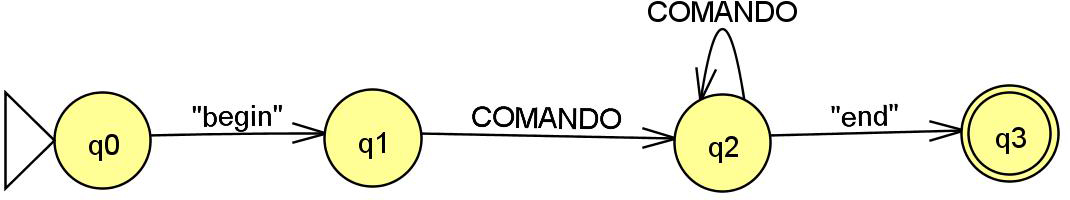
\includegraphics[width=9cm,keepaspectratio]{jflap-automatas/PROGRAMA.jpg}
\caption{\label{fig:programa-jflap} PROGRAMA.jpg}
\end{figure}

\begin{figure}[H]
\centering
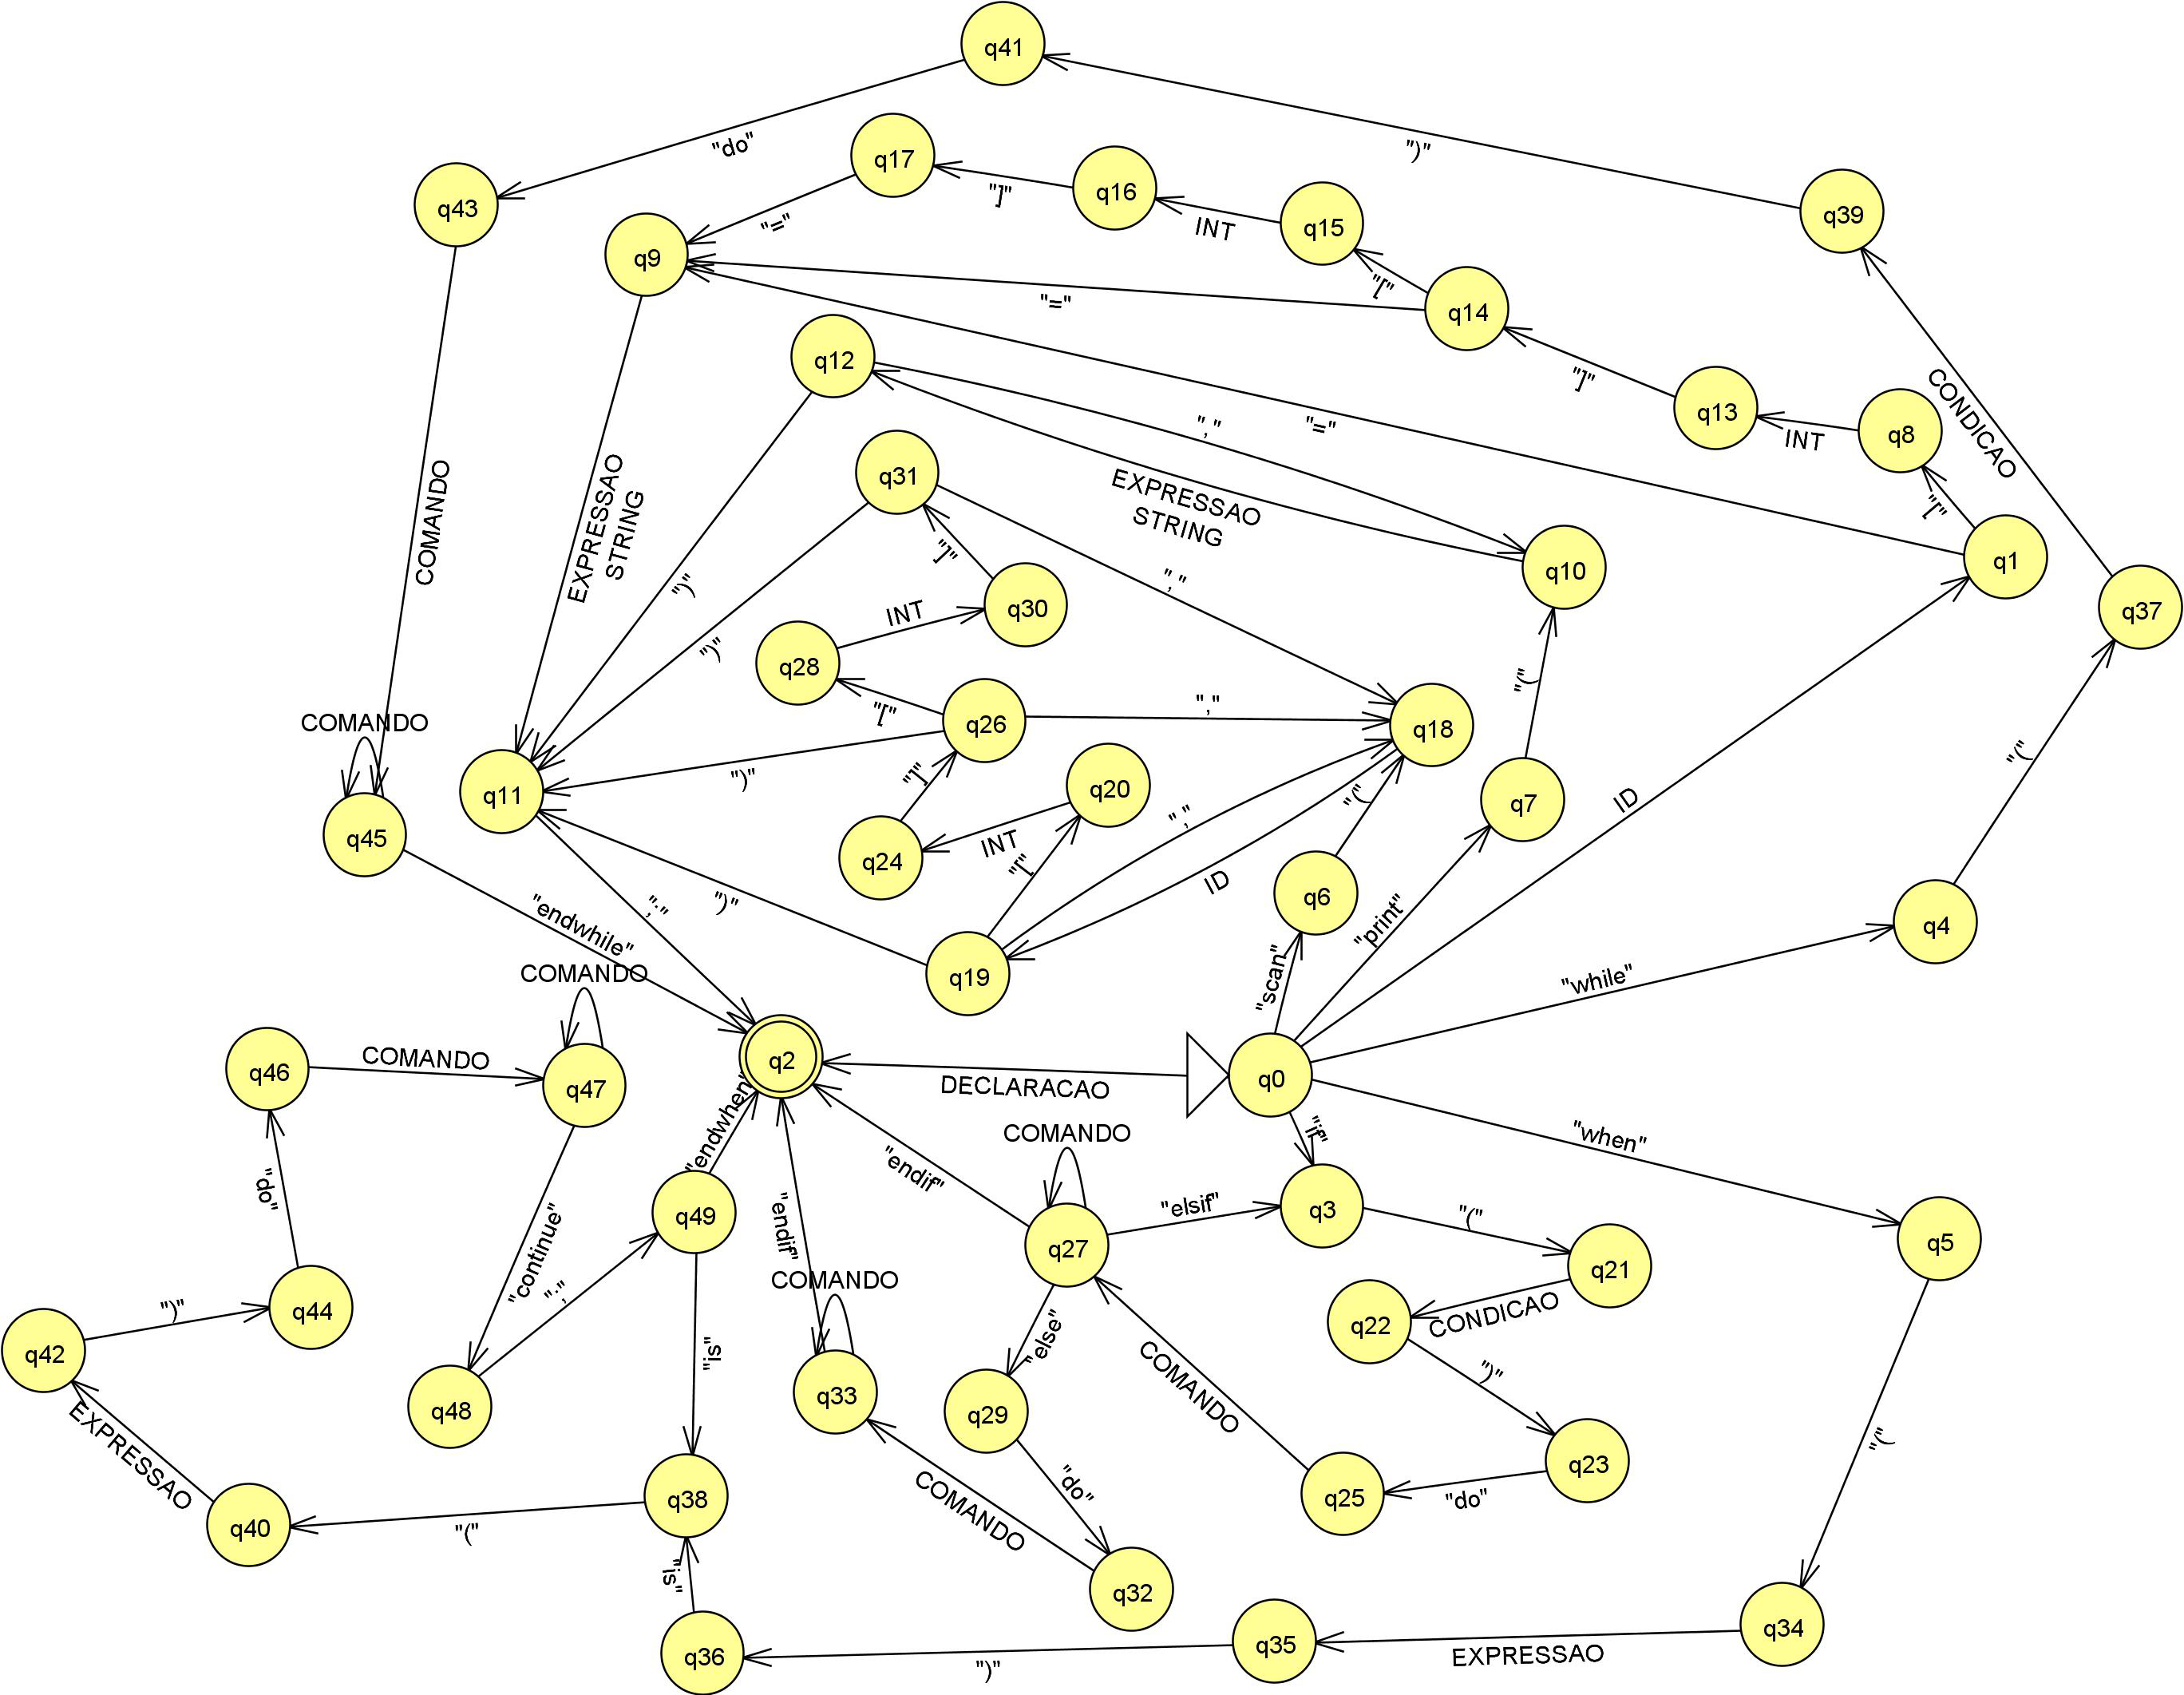
\includegraphics[width=9cm,keepaspectratio]{jflap-automatas/COMANDO.jpg}
\caption{\label{fig:comando-jflap} COMANDO.jpg}
\end{figure}

\begin{figure}[H]
\centering
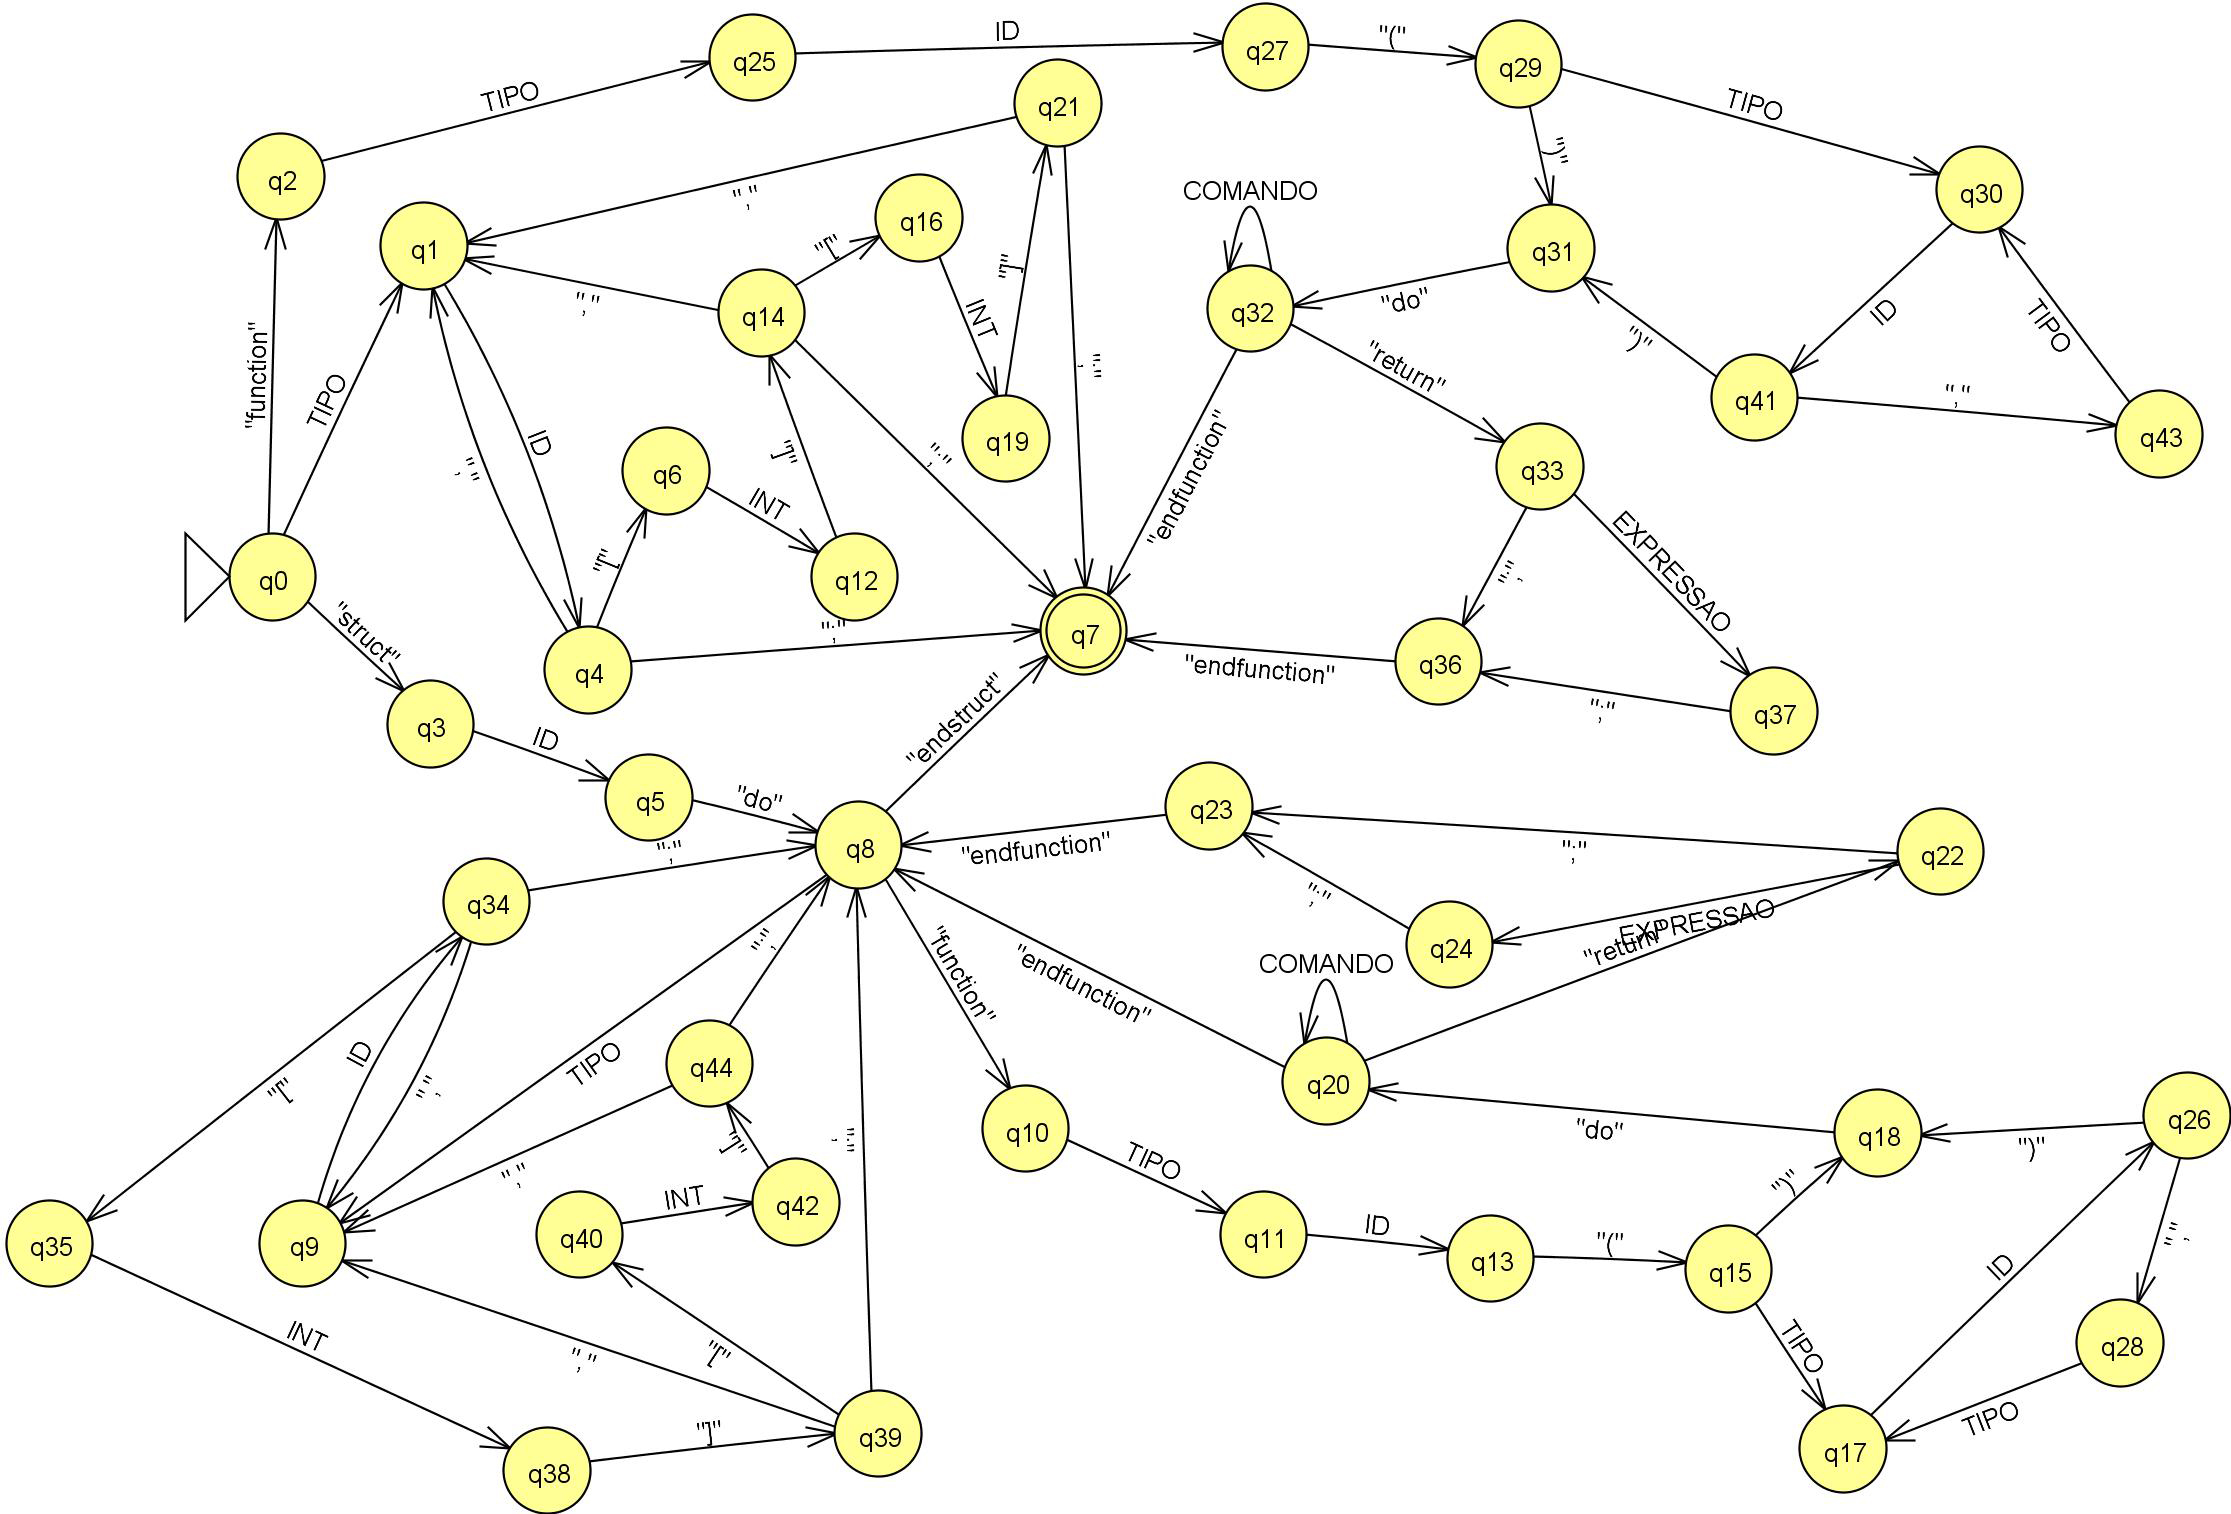
\includegraphics[width=9cm,keepaspectratio]{jflap-automatas/DECLARACAO.jpg}
\caption{\label{fig:declaracao-jflap} DECLARACAO.jpg}
\end{figure}

\begin{figure}[H]
\centering
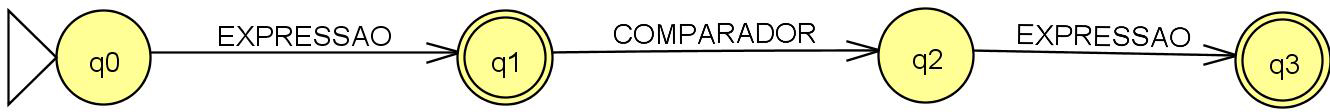
\includegraphics[width=9cm,keepaspectratio]{jflap-automatas/CONDICAO.jpg}
\caption{\label{fig:condicao-jflap} CONDICAO.jpg}
\end{figure}

\begin{figure}[H]
\centering
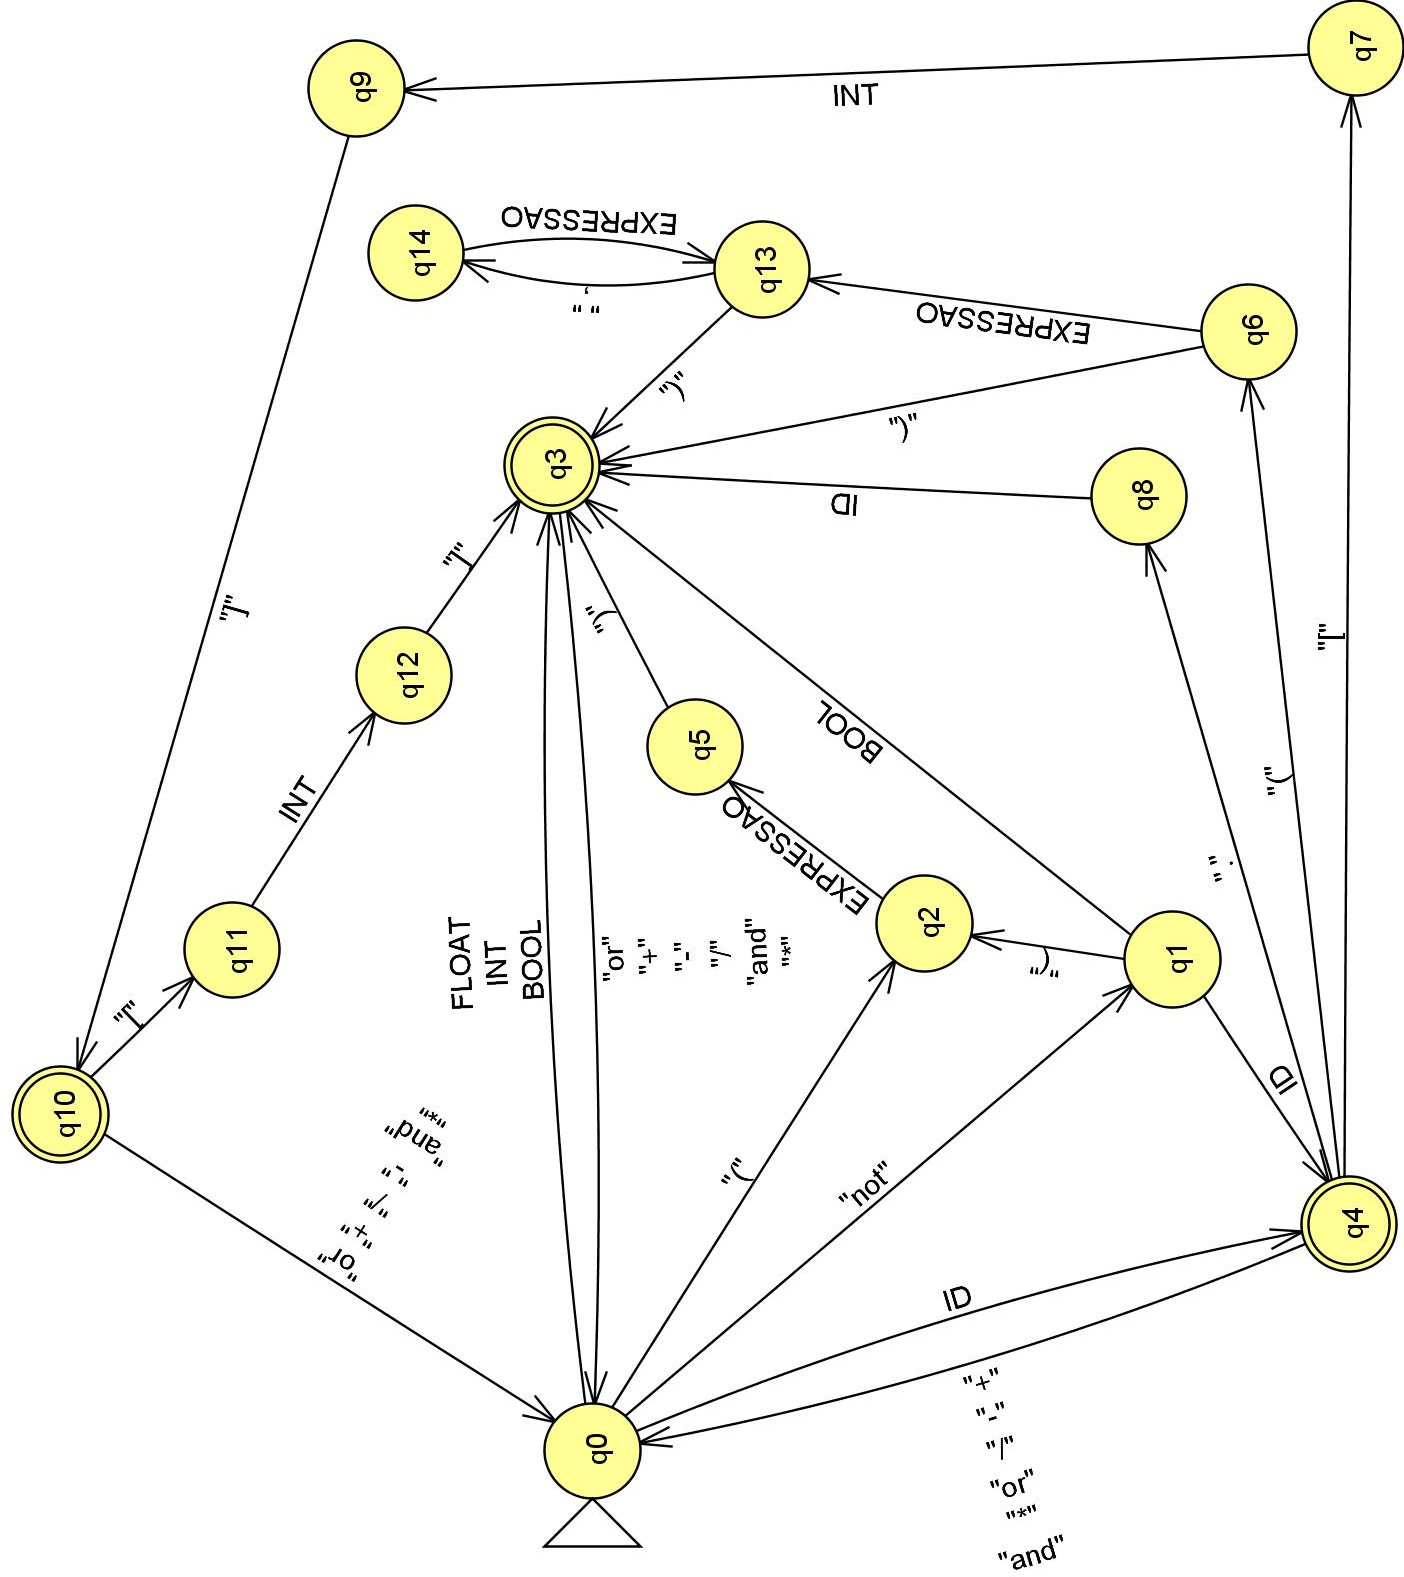
\includegraphics[width=9cm,keepaspectratio]{jflap-automatas/EXPRESSAO.jpg}
\caption{\label{fig:expressao-jflap} EXPRESSAO.jpg}
\end{figure}

\section{Implementação}
Com os automatos de pilha prontos, bastou fazer a implementação. Para isso, foi criado uma struct (AutomataPE) que representa um tipo de monitor. Esse monitor é responsável por gerenciar a pilha (empilhando e desempilhando quando necessário os sub-autômatos), criar os sub-autômatos chamados, e gererenciar as transições dos autômatos. Para isso, são guardadas várias tabelas auxiliares que informam pontos importantes dos autômatos, que foram identificados com um id próprio cada um:
\begin{itemize}
\item transitionTables: Um array de tabelas indexado pelo id da máquina em questão que informa, para cada estado da máquina e token recebido, qual o proximo estado dela; 
\item subMachineCall: Um array de tabelas indexado pelo id da máquina em questão que informa, para o estado atual dessa máquina, qual o id da máquina deve ser chamada. Essas tabelas acabam por ser matrizes-coluna;
\item afterCallStates: Um array de tabelas indexado pelo id da máquina em questão que informa, para a máquina que acabou de ser desempilhada, para qual estado ela deve ir. São tabelas id x id;
\item finalStates:  Um array de tabelas indexado pelo id da máquina em questão que informa, para a máquina em questão quais estados são finais;

\end{itemize}

Com essas informações, falta apenas a lógica para fazer as transições:
primeiramente, deve ser chamada a função initMachines para que sejam inicializadas as tabelas descritas anteriormente. Dessa chamada será retornado um AutomatoPE. Esse deve então ser usado para chamar a função automataPERun, que recebe também o arquivo que contém o programa e um token que será usado de buffer e deve, de inicio, conter o token inicial. Com essas informações, é possível calcular o próximo estado da máquina inicial. Desse ponto são várias as situações possíveis:

\begin{itemize}
  \item Se esse próximo estado não existir na tabela de transição, deve-se investigar se nesse estado é possível chamar alguma máquina;

  \item Se na tabela de chamada de submaquinas existir uma submáquina a ser chamada, basta empilhar a submaquina atual e começar a nova submáquina;

  \item Se na tabela de chamada de submaquinas não existir um id de máquina válido, ainda é possível que o estado em que o autômato reside é final
  \begin{itemize}
	\item Se o estado for final, é necessário desempilhar uma máquina e recomeçar o processo para verificar se o token é reconhecido por máquinas "a cima;
    \item Se o estado não for final, isso significa que o reconhecimento falhou;
    
  \end{itemize}

\end{itemize}

Por causa dessa implementação preditiva (qual deve ser o próximo estado), deve ser dado o primeiro token para começar a operação. E como uma ação de desempilhar e empilhar não envolvem o consumo de token, mas são considerados como um passo do algoritmo, deve-se usar um buffer para não perder tokens já lidos.
